%!TEX root=seke.tex
% mainfile: ../seke.tex

\section{Automated Doubling Experiments}\label{sec:technique}

  \begin{figure*}
    \newcommand{\mx}[1]{\mathbf{\bm{#1}}} % Matrix command
\newcommand{\vc}[1]{\mathbf{\bm{#1}}} % Vector command

% Define the layers to draw the diagram
\pgfdeclarelayer{background}
\pgfdeclarelayer{foreground}
\pgfsetlayers{background,main,foreground}

% Define block styles used later

\tikzstyle{sensor}=[draw, fill=black!20, text width=5em,
    text centered, minimum height=2.5em,drop shadow]
\tikzstyle{ann} = [above, text width=5em, text centered]
\tikzstyle{wa} = [sensor, text width=10em, fill=red!20,
    minimum height=6em, rounded corners, drop shadow]
\tikzstyle{sc} = [sensor, text width=13em, fill=red!20,
    minimum height=10em, rounded corners, drop shadow]

% Define distances for bordering
\def\blockdist{1.5}
\def\edgedist{2.5}

\begin{tikzpicture}
    \node (wa) [wa]  {\textit{SchemaAnalyst}};
    \path (wa.west)+(-\blockdist,-1.0) node (asr1) [sensor] {Database Schema};
    \path (asr1.west)+(-\blockdist,0.0) node (doubler) [sensor] {Schema Doubler};

    \path (wa.west)+(-\blockdist,1.0) node (asr2)[sensor] {Coverage Criterion};
    \path (wa.west)+(-\blockdist,0.0) node (dots)[sensor] {Data Generator};

    \path (doubler.west)+(-\blockdist,-0.0) node (doublera) [sensor] {Schema Doubler};
    \path (dots.west)+(-2.65*\blockdist,-0.0) node (dataa) [sensor] {Data Generator};
    \path (asr2.west)+(-2.65*\blockdist,-0.0) node (criteriona) [sensor] {Coverage Criterion};
    \path (doubler.west)+(-\blockdist,-1.0) node (schemaa) [sensor] {Database Schema};



    \path (wa.east)+(\blockdist,0) node (vote) [sensor] {Test Suite};

    \path [draw, ->] (doubler.east) -- node [above] {}
    	(asr1.180);

    \path [draw, ->] (asr1.east) -- node [above] {}
        (wa.200);
    \path [draw, ->] (asr2.east) -- node [above] {}
        (wa.160);
    \path [draw, ->] (dots.east) -- node [above] {}
        (wa.180);
    \path [draw, ->] (wa.east) -- node [above] {}
        (vote.west);

    \path [draw, ->] (doublera.east) -- node [above] {}
        (doubler.west);
    \path [draw, ->] (dataa.east) -- node [above] {}
        (dots.west);
    \path [draw, ->] (criteriona.east) -- node [above] {}
        (asr2.west);
    \path [draw, ->] (schemaa.east) -| node [above] {}
        (doubler.230);

    \path (vote.east)+(\blockdist,0) node (runtime) [sensor] {Runtime Records};
    \path [draw,->] (vote.east)+(0.3,0) -- node [above]{}
    	(runtime.west);
    \path (runtime.east)+(\blockdist,0) node (runtimeo) [sensor] {Runtime Records};


     \path (vote.east)+(\blockdist,-3.165) node (convalg) [sensor] {Convergence Algorithm};
     \path [draw,->] (runtime.south) -- node [above]{}
    	(convalg.north);
     \path [draw,->] (convalg.west) -| node [above,pos=.25]{Continue Experiment}
    	(doubler.290);

	\path [draw,->] (runtime.east) -- node [above]{}
    	(runtimeo);


    \path (wa.south) +(0,-1) node (asrs) {\textit{SchemaAnalyst} Execution};

    \path (asrs.south) +(0,-1.6) node (singleexp) {Experiment Manager};

    \begin{pgfonlayer}{background}
        \path (doubler.west |- asr2.north)+(-0.3,0.6) node (a) {};
        \path (wa.south -| runtime.east)+(+0.3,-0.6) node (b) {};
        \path (runtime.east |- singleexp.east)+(+0.3,-0.3) node (c) {};

        \path[fill=yellow!20,rounded corners, draw=black!50, dashed]
            (a) rectangle (c);
        \path (asr1.north west)+(-0.2,0.2) node (a) {};

    \end{pgfonlayer}

    \begin{pgfonlayer}{background}
        \path (asr2.west |- asr2.north)+(-0.3,0.3) node (a) {};
        \path (wa.south -| wa.east)+(+0.3,-0.3) node (b) {};
        \path (vote.east |- asrs.east)+(+0.3,-0.3) node (c) {};

        \path[fill=yellow!20,rounded corners, draw=black!50, dashed]
            (a) rectangle (c);
        \path (asr1.north west)+(-0.2,0.2) node (a) {};

    \end{pgfonlayer}



\end{tikzpicture}

    \caption{Technique for conducting automatic doubling experiments.}
    \label{fig:doublingexp}
  \end{figure*}

  Our technique for performing automatic doubling experiments consists of two parts.
  The first is a method for systematically doubling the initial input schema schema,
  and the second is a rule for determining when a conclusion can be
  drawn from the experiment, and the experiment can be stopped.

  \textbf{Doubling Schemas}Determining worst case complexity by doubling
  experiment requires that the size of the input be doubled. A relational database
  schema is a complex artifact with many features and interrelationships.
  This makes determining meaningful doubling rules a non-trivial task.

  % \begin{figure*}
  %   \centering
  %   \centering
  %   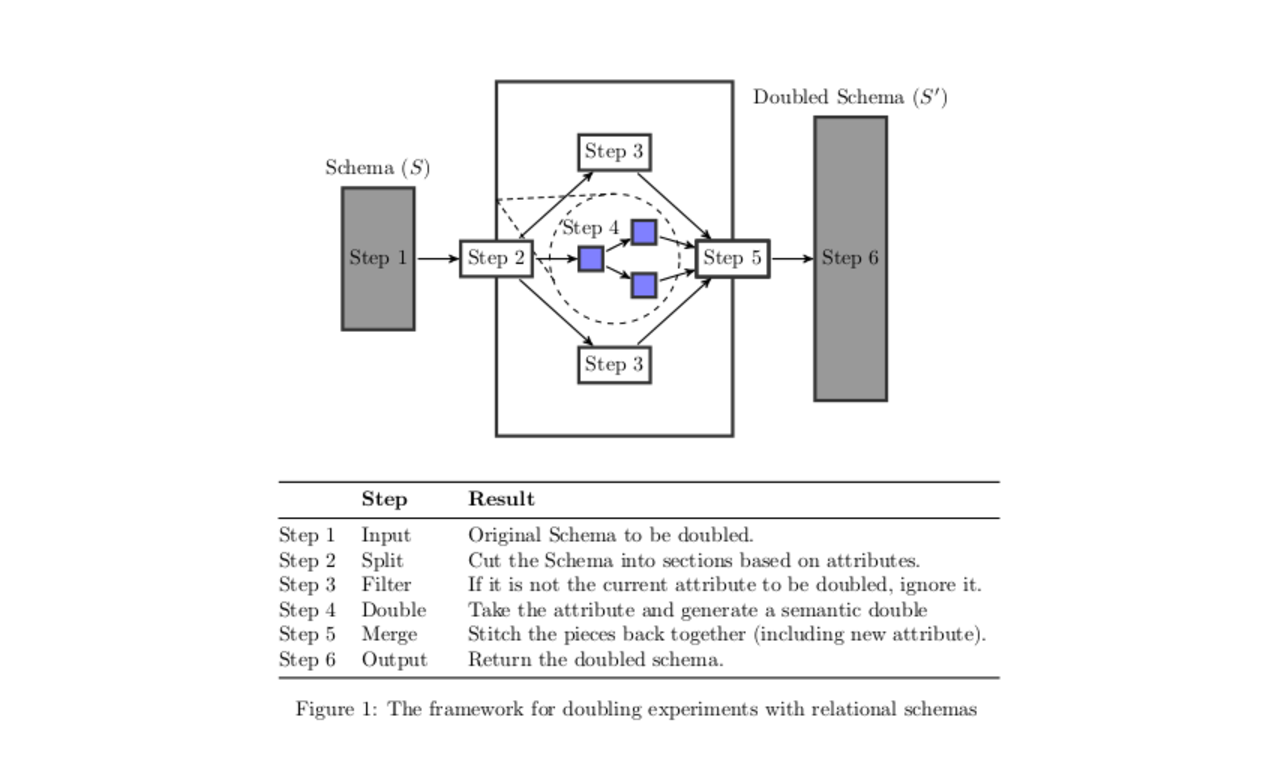
\includegraphics[width=1.25\linewidth]{../diagrams/genDouble}
  %   \caption{Multi Purpose Double Program.}
  %   \label{fig:generaldouble}
  % \end{figure*}

  A relational database schema contains tables, columns, and can contain
  constraints; the runtime of a schema testing tool may be affected by the
  number of any of these. Ideally, we would have a strategy for doubling,
  or a doubler, for each. Doubling the number of tables or columns in a
  schema is relatively easy.  We can double the number of tables in a schema
  by following the rule: for every table present in the schema, we create
  a new empty table. It is important that the new tables be empty to avoid
  changing multiple variables at once.  If the new tables contained
  columns, for instance, then the number of tables and columns in the schema
  would be increased, interfering with our ability to measure the effect of
  tables alone.  Doubling the number of columns can be accomplished by, for
  every table in the schema, for every column, add a new column to that table.
  Doubling integrity constraints is more difficult.  The foreign key
  constraint for instance, donates a relationship between two tables, a check
  constraint can contain arbitrary behavior, and a table can only contain one
  primary key.  If a schema contains five tables, then at most it can only
  have five primary keys.  Adding more keys would require increasing the
  number of tables.  An alternative plan could be starting with a very large
  number of tables with no primary keys that could accommodate doubling their
  number for many trials, but this introduces performance concerns.  Because
  of these issues, we focus our attention to constraints that can be doubled
  as follows: for every table, for every constraint, duplicate that
  constraint and re-add it to the table.  We refer to this doubling strategy
  as, semantic doubling.  Note that constraints doubled this way would not have
  an impact on what data the schema would allow or disallow into a database,
  since semantic doubling amounts to a restatement of existing constraints.
  However, since the goal is to evaluate performance, the results should not be
  affected as long as the test-data generation tool still performs work to
  process the constraints.

  % An example of a general semantic doubling is shown in
  % Figure~\ref{fig:generaldouble}.

  \textbf{Automatic Experiment}To determine worst case complexity, an input
  $n$ is doubled until the ratio $f(2n) / f(n)$ converges to a stable value.
  To account for random error, every time $n$ is doubled, $f(n)$ is recorded
  ten times, and the median time is used for calculating the ratios.  We chose
  median to minimize the effect of outliers. If mean is used instead, a
  single abnormally long run could have a large effect on the result. The
  overall structure of the experiment is shown in Figure~\ref{fig:doublingexp}.

  Convergence checking is necessary because of the fact that worst-case
  time is only apparent for large values of $n$. If too few doubles
  are tried, then the experiment may terminate before $n$ reaches a value
  where the true worst-case time complexity is apparent. At the same time,
  for inefficient  algorithms, each additional doubling run incurs a substantial
  time overhead. For the sake of efficiently, the experiment should
  terminate as quickly as possible.

  To test for convergence, for every time $t$, where $t$ denotes the
  number of times the input has been doubled, we record the each
  doubling ratio $r_t = \frac{f(2^t n)}{f(2^{t-1}n)}$. The current ratio
  $r_c$ is compared to a previous ratio $r_p$ where $p$ is determined by
  a $\mathit{lookback}$ value, such that $p=c-\mathit{lookback}$.  The
  result of the comparison is a $\mathit{difference}$ value, given by
  $\mathit{difference} = |r_c - r_p|$.  This is then compared to a
  tolerance value, and the experiment is judged to have converged when
  $\mathit{difference}<\mathit{tolerance}$.  The $\mathit{lookback}$ and
  $\mathit{tolerance}$ values are both configured before the experiment is
  run.

  Another consequence of worst-case time only being apparent for large
  $n$, is that a very small initial $n$ may appear to converge to one,
  which indicates constant time. To prevent the
  experiment from incorrectly terminating given a small starting $n$, we
  require that a program under study display a ratio of one for a
  $\mathit{minimum}$ number of times before judging that the ratio does in fact converge to one.
  That is, if $r_c = 1$, $t > \mathit{minimum}$ must be true in addition
  to the tolerance test before the experiment is declared convergent.
  The $\mathit{minumum}$ parameter is also configured before an
  experiment.
  Because a doubling ratio of one signifies constant or logarithmic
  time complexity, requiring these doubles does not significantly increase the time needed
  to run the experiment, while providing assurance that a small ratio is not due
  to an insufficiently small $n$.
